\documentclass[12pt]{article}


\usepackage[pdftex]{graphicx}   % assume PDFLaTeX
\usepackage{amsmath}

\textwidth = 6.5 in
\textheight = 9 in
\oddsidemargin = 0.0 in
\evensidemargin = 0.0 in
\topmargin = 0.0 in
\headheight = 0.0 in
\headsep = 0.0 in
%\parskip = 0.2in
\parskip 6pt
\parindent = 0.0in

%\textwidth 6.5in
%\textheight 9in
%\oddsidemargin 0pt
%\evensidemargin 0pt
%\topmargin -.5in
%\headheight .25in

\newtheorem{theorem}{Theorem}
\newtheorem{corollary}[theorem]{Corollary}
\newtheorem{definition}{Definition}
\fontfamily{ptm}\selectfont
\renewcommand{\rmdefault}{ptm}

%\title{Brief Article}
%\author{The Author}
\begin{document}

%\ifpdf
%\DeclareGraphicsExtensions{.pdf, .jpg, .tif}
%\else
%\DeclareGraphicsExtensions{.eps, .jpg}
%\fi

\DeclareGraphicsExtensions{.pdf, .jpg, .tif}



\begin{center}
\section*{Lab 6: Gates and Flip-flops}
UC Davis Physics 116B\\
\end{center}

\section*{Introduction}

In this lab, we will begin by ``looking inside" digital ICs to see how they work. To do this, we will construct simplified models of the circuits they contain.  We will then construct some circuits using standard TTL parts.

\section*{Proto-board}

\begin{figure}[!h]
\centerline{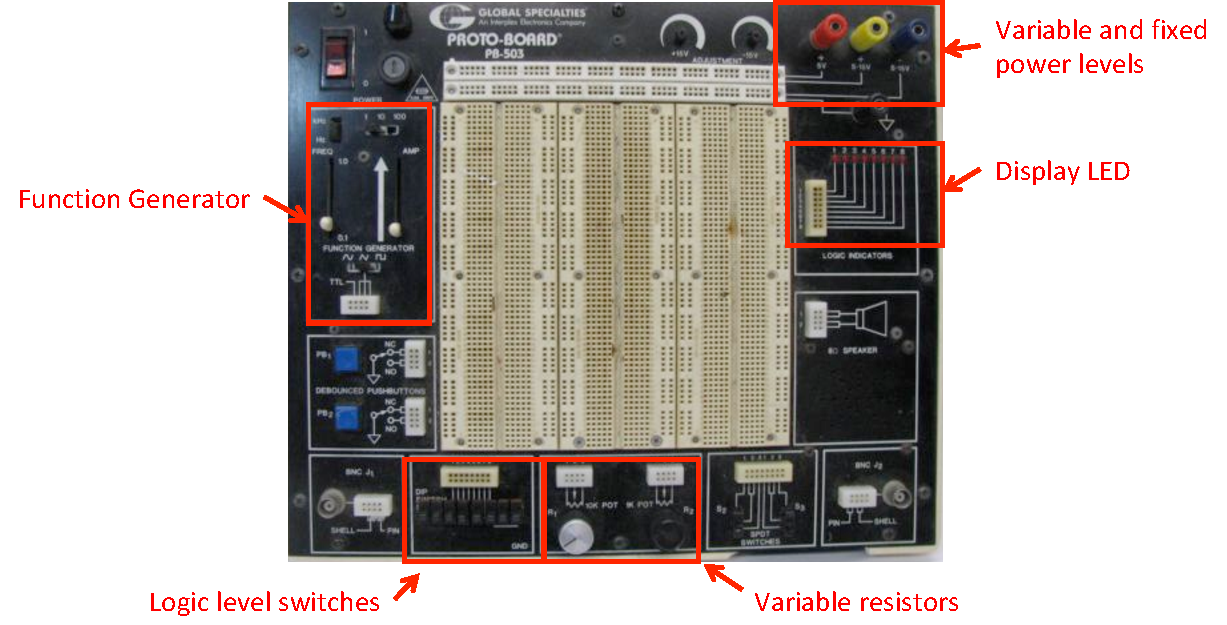
\includegraphics[width=7in]{figs/proto-board.pdf}}
\caption{Proto-board used for digital circuit labs}
\label{fig:proto-board}
\end{figure}

For next few labs, we'll use the older PB-503 proto-boards, shown in Figure~\ref{fig:proto-board}.  They have the advantage of having built-in power supplies, pulse generators, logic switches, and LED displays.  

For the circuits in this lab, you can use the switches to set the logical state of the inputs, and the LEDs to display the logical state
of the outputs. For the next few labs, always set the switch level selector to ``TTL" and the LED level selectors to ``+5V" and ``TTL" to insure the correct logic levels! 

\section*{RTL Circuits}

\begin{figure}[!h]
\centerline{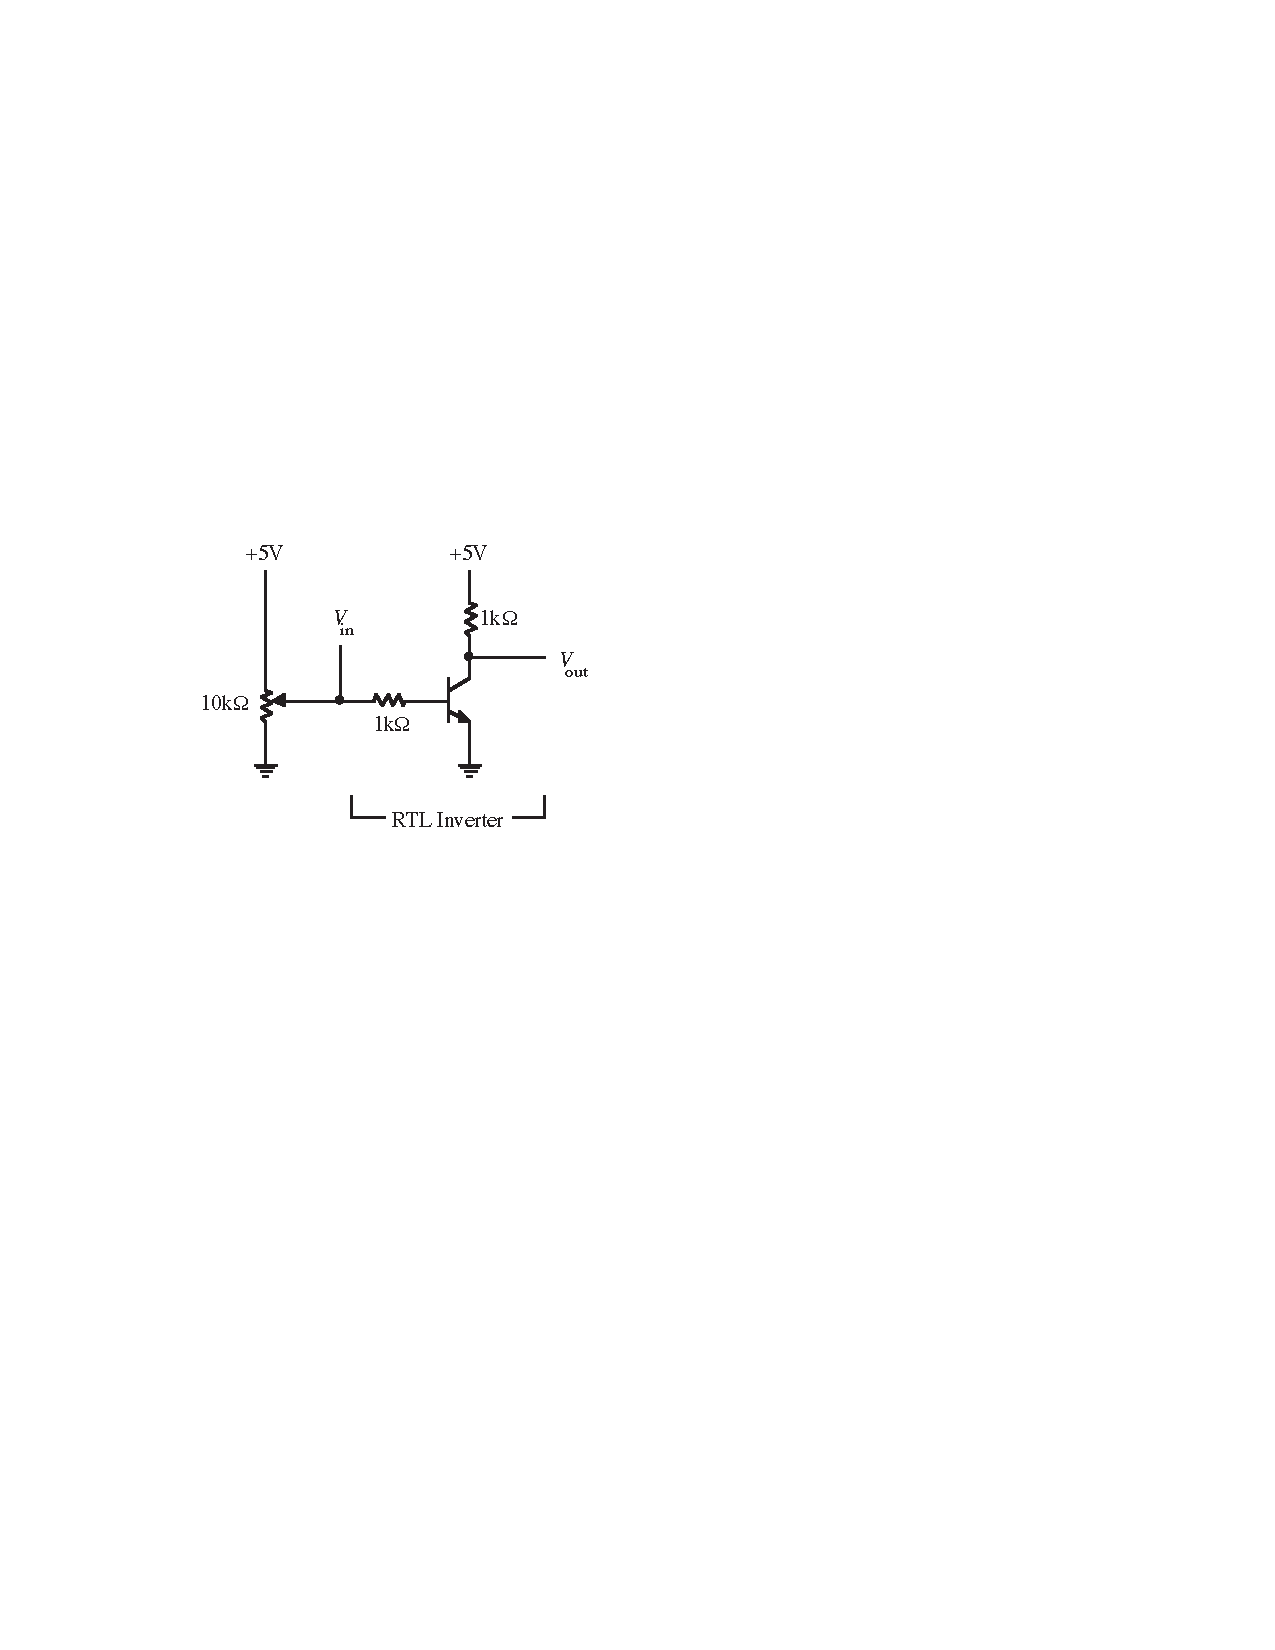
\includegraphics[width=3in]{figs/inverter.pdf}}
\caption{A logical inverter implemented in RTL.}
\label{fig:inverter}
\end{figure}

\begin{figure}[!h]
\centerline{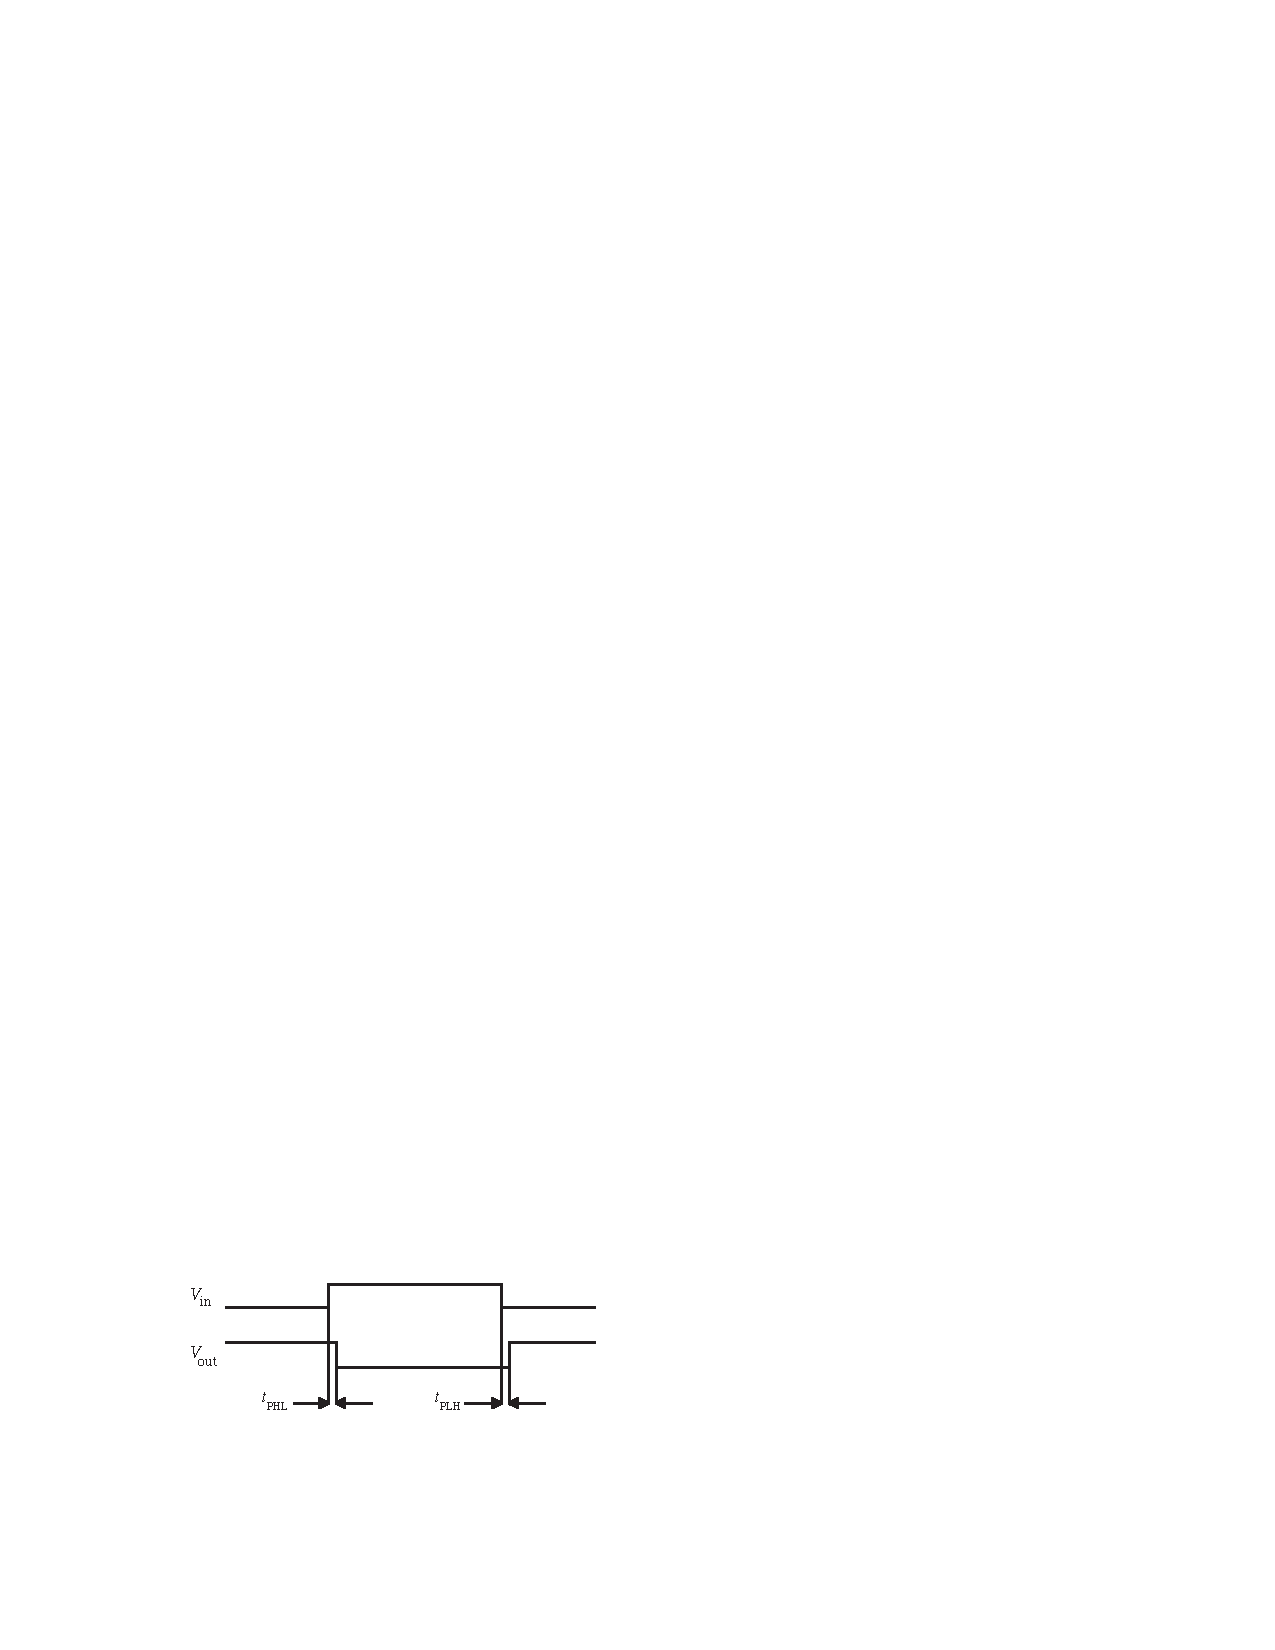
\includegraphics[width=3in]{figs/propagation.pdf}}
\caption{Propagation of the signal inversion.}
\label{fig:propagation}
\end{figure}

\begin{figure}[!h]
\centerline{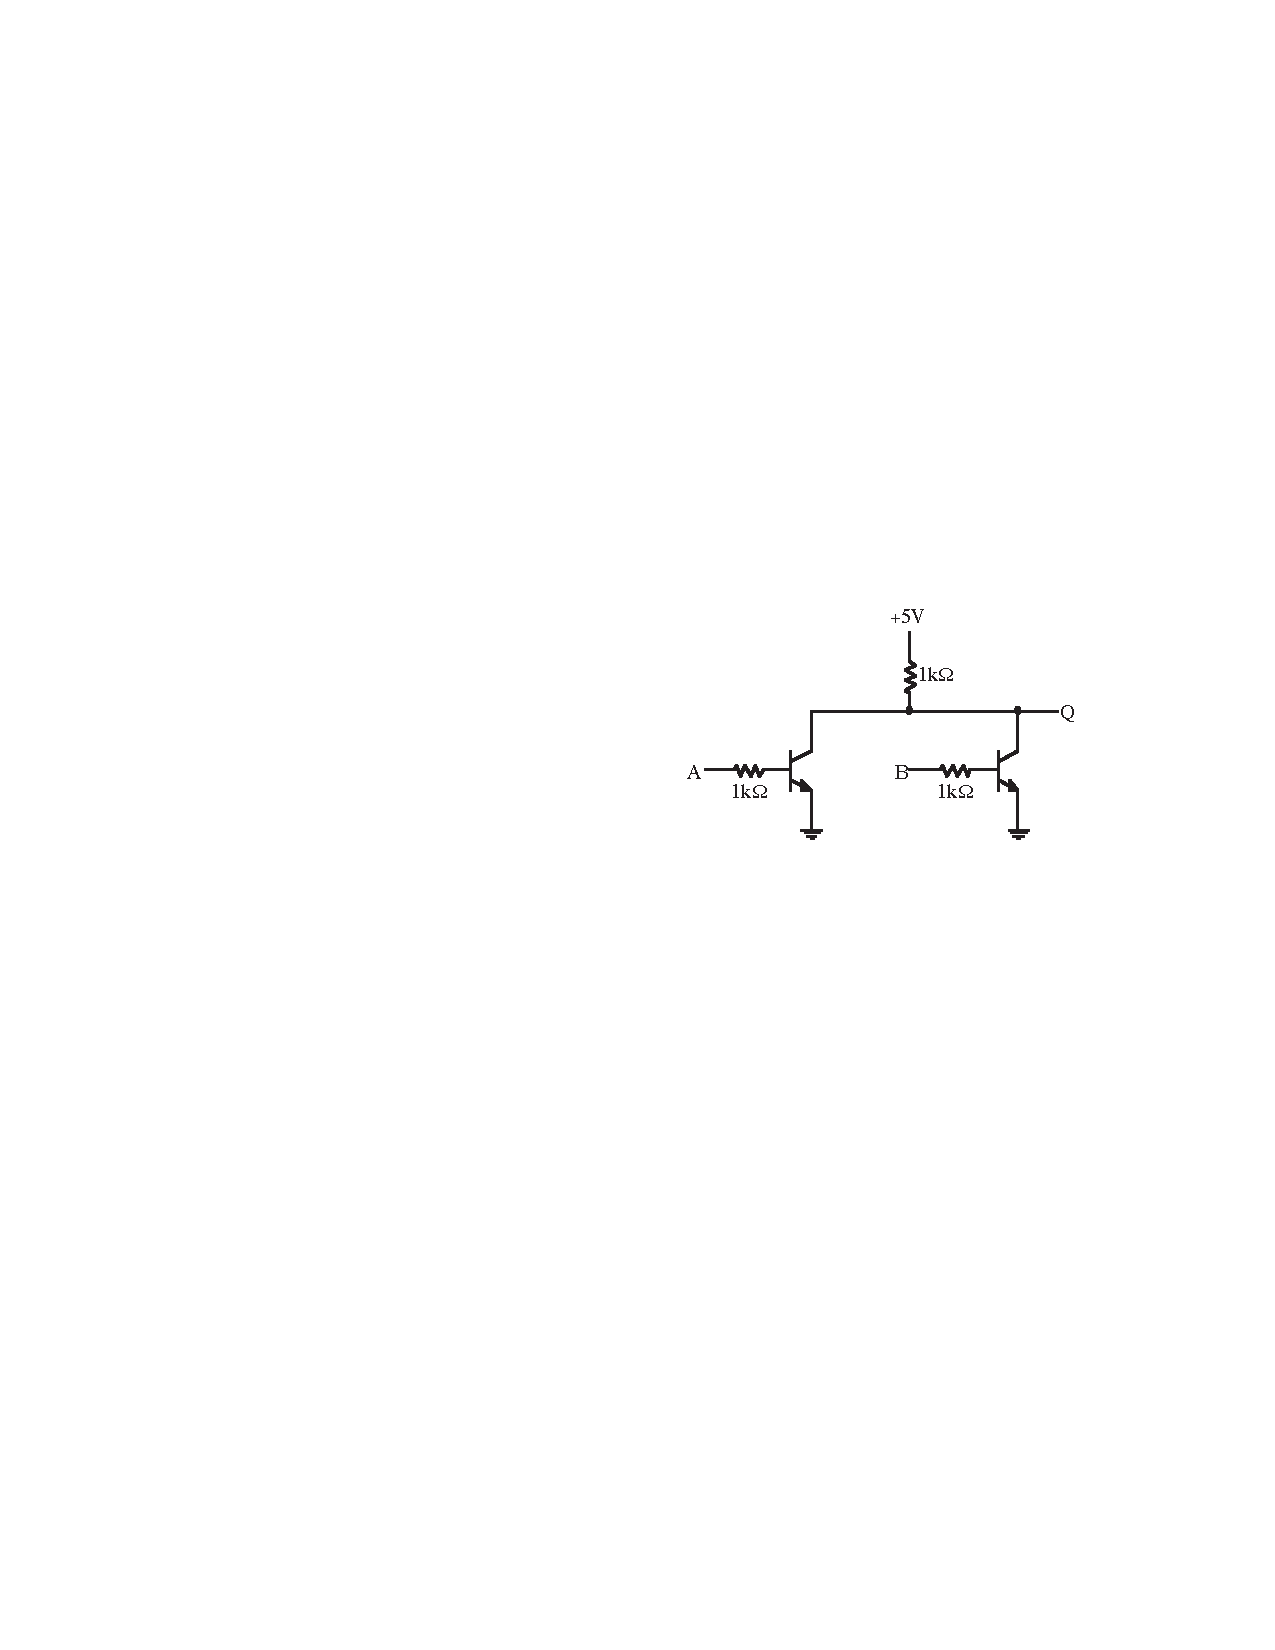
\includegraphics[width=3in]{figs/RTL-NOR.pdf}}
\caption{NOR gate implemented in RTL.}
\label{fig:RTL-NOR}
\end{figure}

``Resister Transister Logic" (RTL) is a way to implement logic using discrete components, and it's very similar to the way
``Transistor Transistor Logic" (TTL) chips work internally.  

\subsection*{Inverter}

Construct the RTL inverter circuit shown in Figure~\ref{fig:inverter}, using a 2N3904 NPN transistor. Note that the input is an analog voltage from built-in  potentiometer for now. For your lab report, make a graph of $V_{out}$ vs. $V_{in}$. Use this graph to describe the function of an inverter; that is, what must a circuit do to invert a logic signal?

Now disconnect the potentiometer and connect the input of the inverter to a logic switch and the output to an LED monitor. Does it function as an inverter?  Remember, for logic circuits, we only care about the behavior for a 0 (LOW) or 1 (HIGH) input, not the behavior for intermediate values.

Now drive the input with the ``TTL"  output (5V square wave) of the function generator on the proto-board at about 10 kHz.  Look at the input and output on the oscilloscope. The output should be the inverse of the input with a small time delay as shown in Figure~\ref{fig:propagation}.  

Using the vertical cursors on the scope, measure the propagation delays $t_{PHL}$ (the time for the output to change
from high to low) and $t_{PLH}$ (low to high). Propagation delay is the main enemy of fast
circuits; minimizing it is the goal of most device engineers. Which propagation delay is shorter? Can you guess why? For your lab report, include the oscilloscope trace and answer the questions.


\subsection*{NOR Gate}

Now modify your inverter to be a NOR gate with inputs A and B and output Q as shown in Figure~\ref{fig:RTL-NOR}. Drive the inputs with the switches and connect the output to an LED. Verify that this is indeed a NOR gate by experimentally constructing its truth table for all combinations of inputs.


\section*{Standard TTL Chips}


\begin{figure}[!h]
\centerline{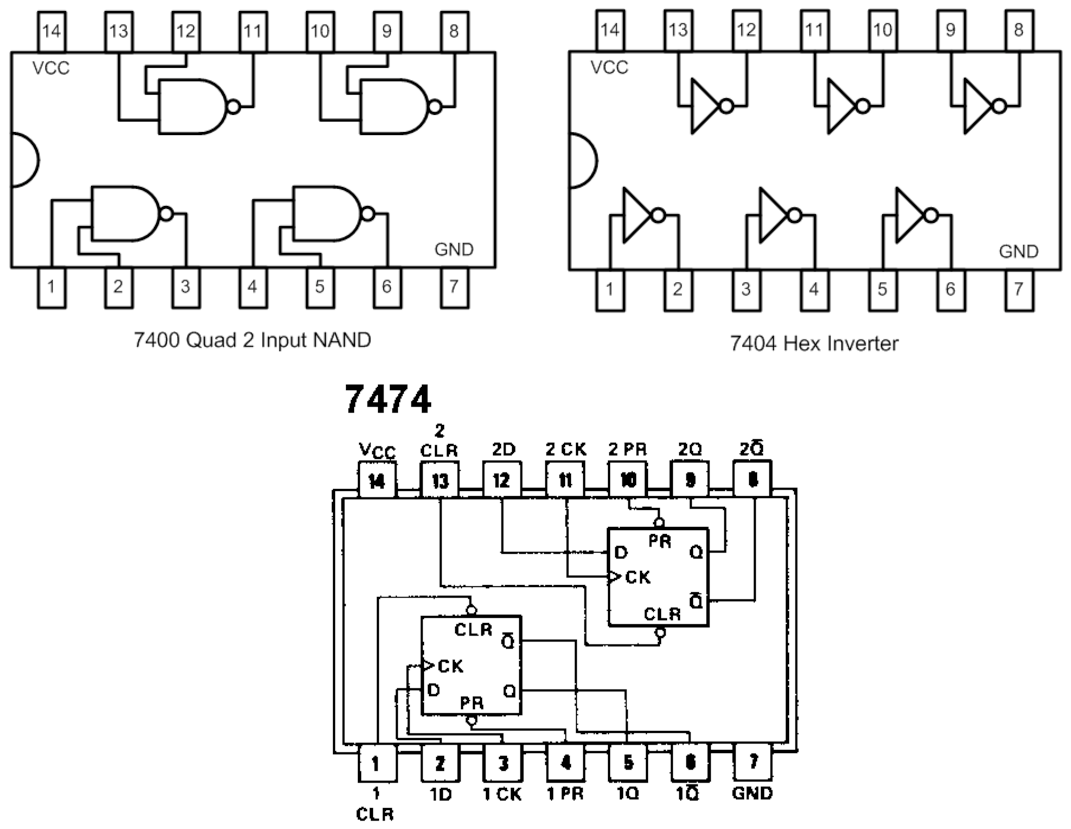
\includegraphics[width=5in]{figs/chips.pdf}}
\caption{Pinouts for TTL chips used in this lab: 74LS00, 74LS04, and 74LS74.}
\label{fig:chips}
\end{figure}

For many years, most digital logic was constructed using standard logic chips, and those are what we'll be using for the next few labs.  
Figure~\ref{fig:chips} shows the chips we'll be using for this lab:
\begin{itemize}
\item{\bf 74LS00:} Quad NAND gate.
\item {\bf 74LS04:} Hex inverter.
\item {\bf 74LS74:} Dual D-latch.
\end{itemize}

Note that for all N-pin TTL chips, pin-$N$ is connected to +5V and pin-$\frac N2$ is connected to GROUND.  For example, all of these are 14-pin chips, so pin 14 is connected to +5V and pin 7 is connected to GROUND. 

\section *{Data Latch}

You will now construct a D flip flop (a memory circuit) in several steps.
\subsection*{SR Flip Flop with Discrete Gates}
First, construct the SR (set-reset) latch shown in Figure~\ref{fig:flip-flop} using two of the NAND gates in the 74LS00. Verify the truth table for this circuit and explain why Q can be either 1 or 0 when $\bar S$ and $\bar R$ are both 1. Draw a time line diagram to illustrate how this circuit works as a memory device.


\begin{figure}[!h]
\centerline{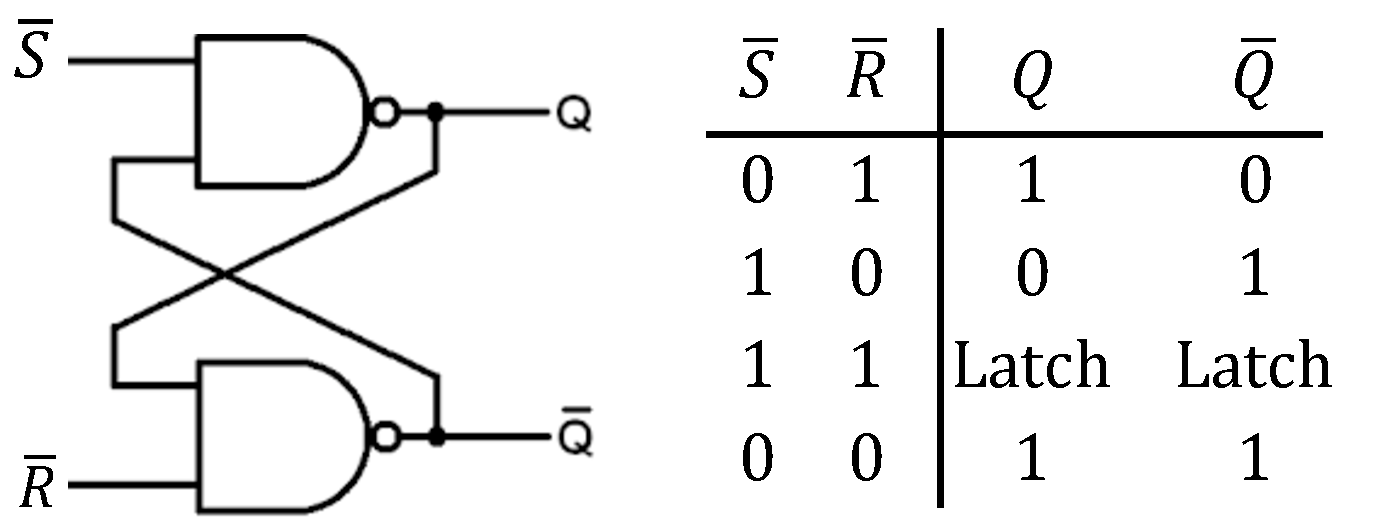
\includegraphics[width=3in]{figs/flip-flop.pdf}}
\caption{SR flip flop implemented out of discrete gates, with associated truth table. ``Latch" means 	``remains in current state".}
\label{fig:flip-flop}
\end{figure}

\subsection*{Data Latch with Discrete Gates}

Now modify the SR latch with the remaining two gates in the 74LS00 to have a gated data input as shown in Figure~\ref{fig:d-latch}. This is the ``transparent latch" circuit. Construct a truth table for this circuit and explain its operation using a time line diagram as you did for the SR latch.

Use the 74LS04 and a second 74LS00 to construct the rather crude edge trigger shown in Figure~\ref{fig:edge}. Drive it with the TTL output from the 
function generator, and use the scope to measure the width of the output pulse.  Include this in your report. 

Once you have verified the edge trigger works, connect the input to one of the logic switches and the output
to the $C$ input of your latch circuit.  
The complete circuit you now have should function like  the  D flip flop shown in Figure~\ref{fig:d-latch-part}. Verify 
that regardless of the state of $D$, $Q$ will only change when $CLK$ transitions from 0 to 1.
Construct a truth table for this circuit and draw a time line diagram to illustrate this.  Note that the symbol for ``rising edge" 
in a truth table is an upward arrow ($\uparrow$).  Be sure your truth table includes entries for all $CLK$ states ($1,0,\uparrow,\downarrow$).

\begin{figure}[!h]
\centerline{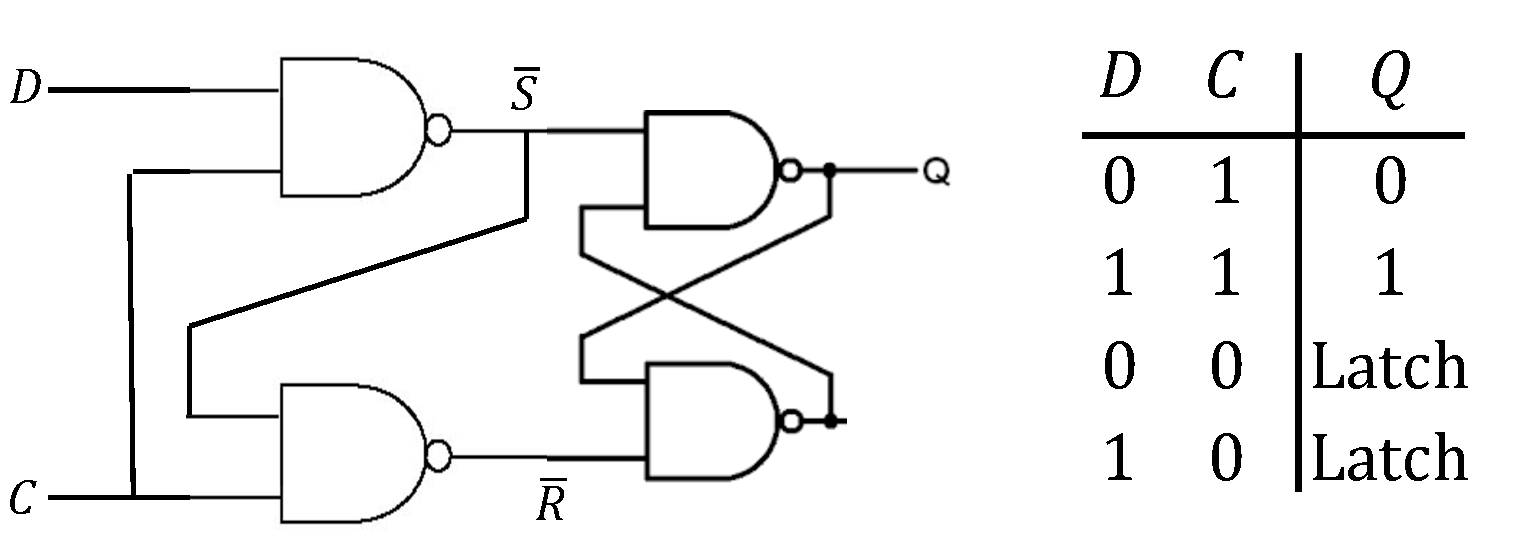
\includegraphics[width=4in]{figs/d-latch.pdf}}
\caption{Data latch implemented with discrete parts.}
\label{fig:d-latch}
\end{figure}

\begin{figure}[!h]
\centerline{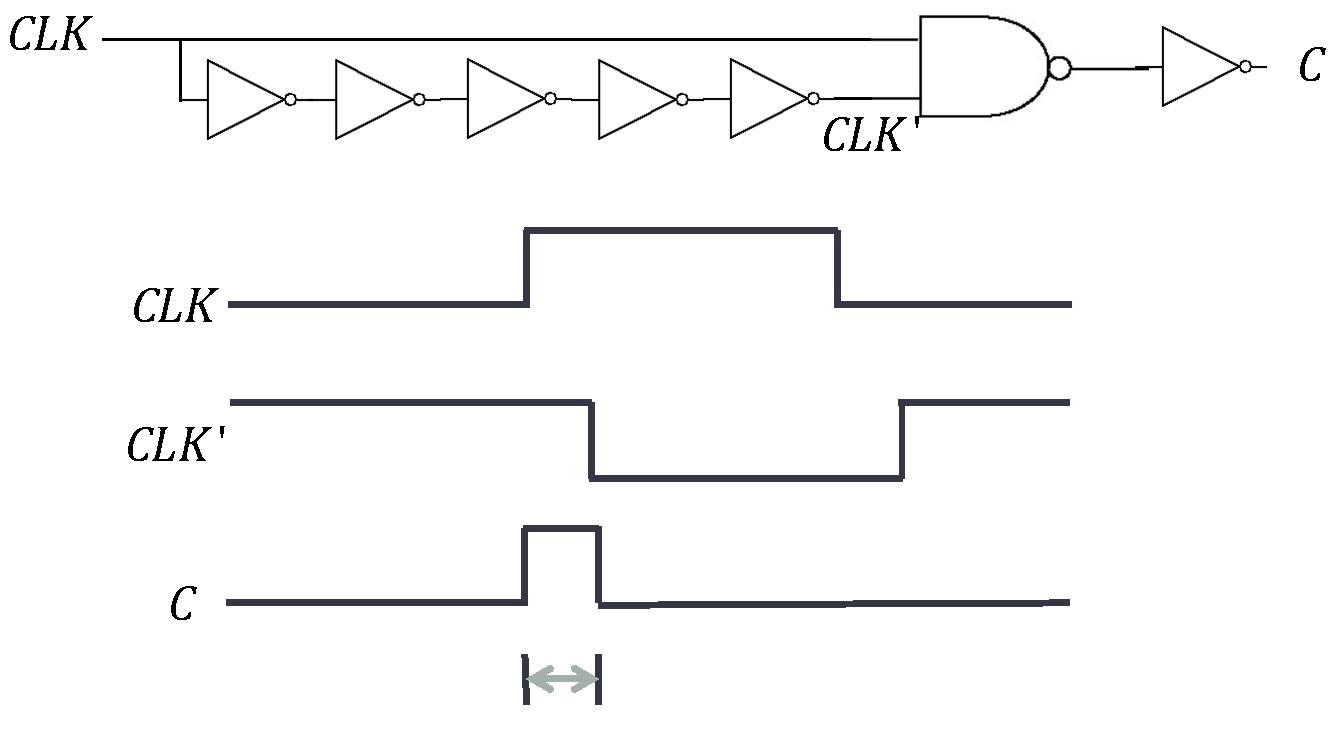
\includegraphics[width=5in]{figs/edge.pdf}}
\caption{Generating an edge tigger.}
\label{fig:edge}
\end{figure}

\begin{figure}[!h]
\centerline{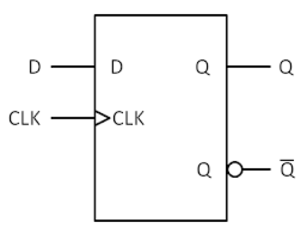
\includegraphics[width=2in]{figs/d-latch-part.pdf}}
\caption{Behavior of the circuit that we've constructed.}
\label{fig:d-latch-part}
\end{figure}

\subsection*{Standard Data Latch}
\begin{figure}[!h]
\centerline{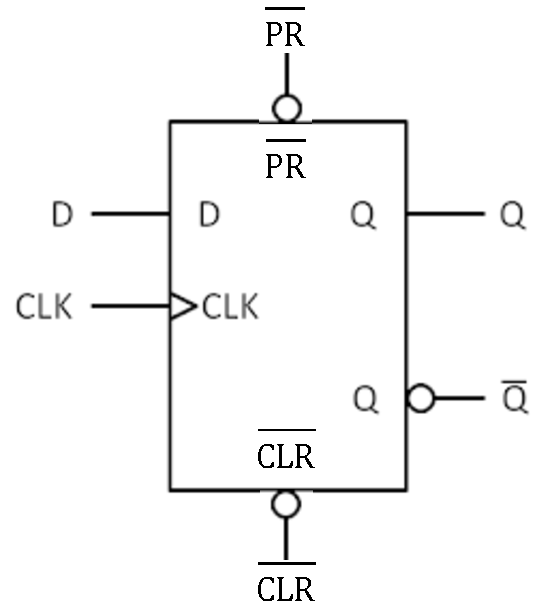
\includegraphics[width=2in]{figs/d-latch-7474.pdf}}
\caption{Standard data latch with asynchronous preset and clear.}
\label{fig:d-latch-7474}
\end{figure}

Data latches are an important part of synchronous logic designs, so rather than construct them out of discrete logic gates, 
they are implemented as standard parts.  For example, the 74LS74  contains two data latches with the 
inputs and outputs shown in Figure~\ref{fig:d-latch-7474}.  In addition to the inputs we discussed in the previous section,
each of these has  asynchronous preset ($\overline{PR}$) and clear ($\overline{CLR}$) which will set or clear the output, regardless of the state of $D$ or $CLK$.

We will be building synchronous logic circuits with these in future labs.



\end{document}



